\chapter{CAMION: Catchment Area MaximizatION algorithm}

\section{Context}

\subsection{Motivation}

Uneven distributions of population and health-care providers lead to geographic disparity in accessibility for patients \cite{wang_why_2020}. For instance, Weiss et al. \cite{weiss_global_2020} showed that 8.9\% of the global population could not reach healthcare within one hour if they have access to motorized transport. In Germany, Bauer et al. \cite{bauer_spatial_2020} shown that 10\% of the population lived in areas with low accessibility for internal medicine and surgery. Location-allocation algorithms \cite{church_location_1999} can optimize the distribution and supply of health providers to reduce accessibility disparities. These algorithms seek the optimal placement of facilities for a desirable objective under certain constraints \cite{wang_measurement_2012}. For instance, Luo et al. developed an optimization algorithm to improve the healthcare planning in rural China by finding the best place and capacity for new health facilities \cite{luo_integrating_2014}. Tao et al. worked on a spatial optimization model to maximize equity in accessibility to residential care facility in Beijing, China \cite{tao_spatial_2014}. When optimizing health accessibility, there are two competing goals: equity and efficiency \cite{krugman_opinion_2013,meyer_equity_2008}. Equity may be defined as equal access to healthcare for everyone \cite{culyer_equity_1993}. An efficient situation is when everything has been done to help any person without harming anyone else \cite{hemenway_optimal_1982}. While some argue that efficiency should be ad-dressed in priority \cite{hemenway_optimal_1982}, others agree that equity is a matter of ethical obligation, especially in public health \cite{fried_rights_1975, oliver_equity_2004}.

\subsection{Location-allocation algorithms}

Regarding efficiency optimization, the most popular algorithms are p-median, location set covering problem (LSCP) and maximum covering location problem (MCLP). The p-median algorithm minimizes the weighted sum of distances between users and facilities \cite{murad_using_2021}. LSCP minimizes the number of facilities needed to cover all demand \cite{shavandi_fuzzy_2006}. MCLP maximizes the de-mand covered within a desired distance or time threshold by locating a given number of facilities \cite{casado_heuristical_2005}.
To reach equal access to healthcare, quadratic programming has been used to  minimize the variance of accessibility scores defined by the 2SFCA \cite{wang_planning_2013}. Similarly, a Particle Swarm Optimization (PSO) algorithm was developed to minimize the total square difference between the accessibility score of each demand location and the weighted average accessibility score \cite{tao_spatial_2014}. Finally, a two-step optimization algorithm has been developed to address the dual objectives of efficiency and equality, by first choosing where to site new hospitals and then deciding which capacity they should have \cite{luo_two-step_2017,li_two-step_2017}.

\section{Methods}

However, most of the previous algorithms seek locations to open new health facilities. In this work, we are interested in the case where the health facilities are fixed, and the only lever to improve accessibility is to increase their capacities. Given a capacity budget, we want to know which facilities to grow and by how much. We introduce CAMION, an accessibility optimization algorithm based on Floating Catchment Area and Linear Programming. The initial accessibility score was computed with the Enhanced Two Step Floating Catchment Area (e2SFCA) \cite{luo_enhanced_2009} but our algorithm can generalize to more FCA derivatives.
We model the problem as an optimization task. In our case, we want our optimization algorithm to find new care centers capacities given some constraints, so that the total accessibility is maximum. We apply optimization on a given region only, rather than on the whole metropolitan France. We chose this approach because healthcare planning is handled regionally rather than nationally. We show below that our optimization problem is a Linear Programming problem.
In its standard form, Linear Programming finds a vector $x$ that maximizes $c^T x$ under constraints $Ax \leq b$, where $A$ is a matrix and $b$ a vector. Boundaries can be set to $x$ such as $x \geq 0$. Consider $x_u$ the new capacity of a care center $u$, to be computed by the algorithm. Let $Q_u$ and $W_u$ be two vectors of size $m$, defined as follows:

\begin{align}
    Q_u &=  \sum_{s=1}^{r} W_s \sum_{i, d_{iu} \in I_s} P_i \\[10pt]
    W_u &=  \sum_{s=1}^{r} \sum_{i, d_{iu} \in I_s} W_s
\end{align}

We can compute the total accessibility as a sum on the m care centers:

\begin{align*}
    \sum_{i} A_i &= \sum_{i} \sum_{s=1}^{r} W_s \sum_{u, d_{iu} \in I_s} \frac{S_u}{Q_u} \\[10pt]
    \sum_{i} A_i &= \sum_{i} \sum_{i, d_{iu} \in I_s} W_s \frac{S_u}{Q_u} \\[10pt]
    \sum_{i} A_i &= \sum_{u} \frac{S_u}{Q_u} \sum_{s} \sum_{i, d_{iu}} W_s \\[10pt]
    \sum_{i} A_i &= \sum_{u} \frac{S_u}{Q_u} W_u \numberthis \label{eq:A_i_sum_u}
\end{align*}

\cref{eq:A_i_sum_u} can be rewritten in the Linear Programming standard form with:

\begin{align*}
c &= \frac{W_u}{Q_u} \\
x_u &= S_u  \\
b &\geq \sum_{u} x_u  \\
x_{u_\text{min}} &\leq x_u \leq x_{u_\text{max}}
\end{align*}

The user-defined parameters are $b$, $x_{u_\text{min}}$ and $x_{u_\text{max}}$. $b$ is the total capacity to be shared across all the care centers. $x_{u_\text{min}}$ and $x_{u_\text{max}}$ are the capacity boundaries for care center $u$. If $b$ is set to the current total capacity, a care center can’t be grown unless another one is decreased. If $b > \sum_{u} x_u$, the capacity of care centers can be increased without decreasing other centers. We know how to solve Linear Programming and we used the SciPy \cite{virtanen_scipy_2020} implementation of the revised simplex method as explained in \cite{bertsimas_introduction_1998}.
We now detail how we set the user-defined parameters to apply the Linear Programming algorithm to our specific case. The additional capacity was set as +3\% of the overall activity of the region's care centers: $b = 1.03 \times \sum_{u} x_u$. The choice of the boundaries $x_{u_\text{min}}$  and $x_{u_\text{max}}$ is crucial and must be realistic. We studied the hospitals activity on the past four years (2016 to 2019) to retrieve the average growth percentage of a care center. The growth percentage is computed as follows: $(S_\text{2019} - S_\text{2016}) / S_\text{2016}$ . Among the care centers that grew and who had an existing oncology activity, the mean growth percentage was 23\%. Hence, we set $x_{u_\text{max}}$ as +20\% of the care center capacity. Regarding $x_{u_\text{min}}$, we set the boundary based on the cluster of the care center. For the three most specialized clusters, we set their $x_{u_\text{min}}$ equal to their current activity. We did this to prevent the algorithm from decreasing the most specialized and well-equipped care centers. Regarding the care centers from the other clusters, $x_{u_\text{min}}$, so that they could be emptied if need be. Finally, we set $x_{u_\text{max}}$ if the care center belongs to the least specialized cluster. The new capacities are indicative and should be further investigated to make sure they are relevant. Especially when setting an existing oncology activity to 0.

\section{Results}

\begin{figure}[t]
    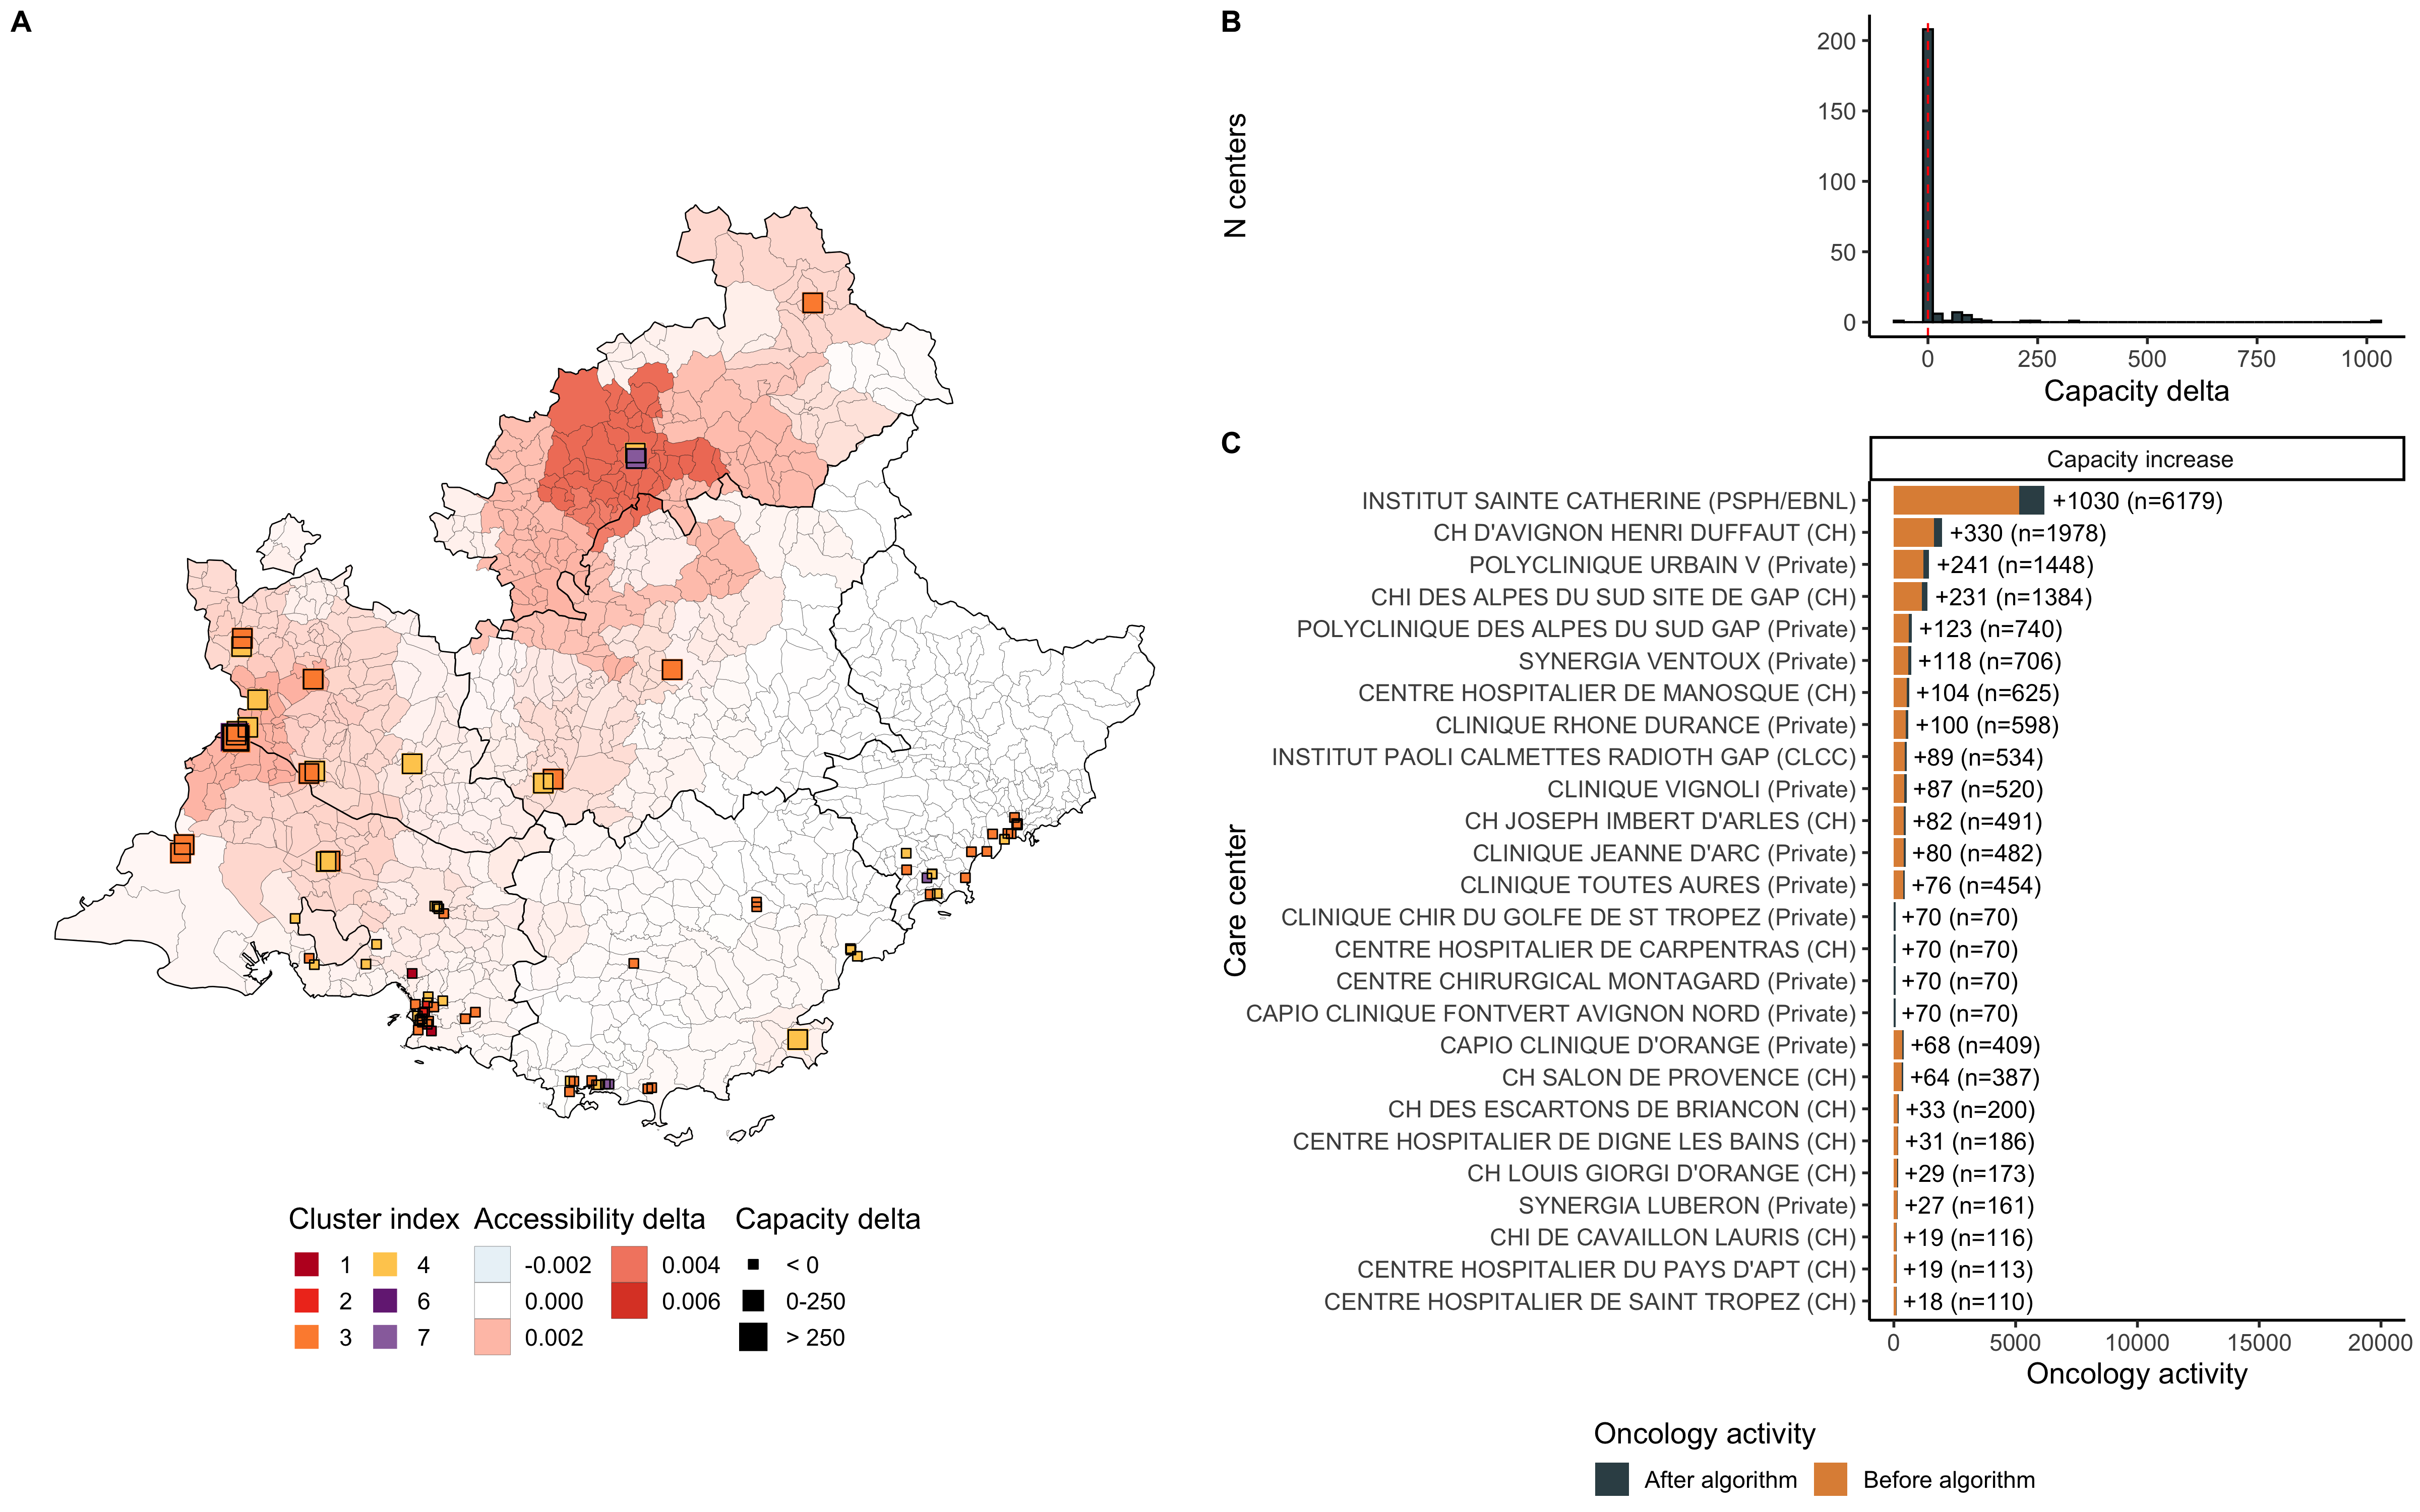
\includegraphics[width=\textwidth]{images/camion/fig5_Provence-Alpes-Cote-d'Azur.png}
    \centering
    \caption{
        Accessibility delta in Provence-Alpes-Cote-d’Azur (PACA) region after running the optimization algorithm. Map (A) displays the accessibility delta ($A_{i_\text{after}} - A_{i_\text{before}}$) by municipality. Plot (B) shows the capacity delta ($S_{u_\text{after}}-S_{u_\text{before}}$) distribution. Capacity was defined as the oncology activity: the number of patients with chemotherapy or radiotherapy and the number of medical or surgery stays related to oncology. We show the list of the care centers that grew the most (C)  and by how much. For instance, the hospital Institut Sainte Catherine in Avignon, was assigned a +1,030 capacity, for a total of n=6,179. Additional activity was 3,221. 26 centers grew and 1 decreased. Median accessibility before optimization was 0.0093 and 0.0103 after, corresponding to a 11.1\% increase.  Accessibility increased around cities like Avignon and Gap. Care centers near Nice were left unchanged by the algorithm.
    }
    \label{fig:optim-paca}
\end{figure}

\section{Web application}

We developed a web application that allows the users to run the optimization algorithm in any region with the parameters they want. The application displays accessibility results and optimization outcomes on an interactive map with additional plots. The user can browse the list of care centers by cluster and the list of municipalities with their accessibility scores.

\section{Discussion}

The quality of oncology care is linked with the care centers' volume. A care center with a very low activity is less likely to provide decent care. As a result, the French National Institute of Cancer (INCa) defined several thresholds (36) that forbid care centers with very low activity to keep operating. Similarly, the care quality in a saturated care center won’t be good either, since patients are more likely to wait longer before diagnosis or between interventions. While it is easy to spot care centers with low activity, it is harder to judge if a care center is over-crowded, and we should be careful when attributing new activity to the hospitals. We based the 20\% max growth out of the previous centers’ activity increase. This percentage could be tailored to the center cluster or current activity. Volume is not the only factor determining care quality. More sophisticated indicators like average delay between diagnosis and first treatment can tell whether a care center is in line with the care pathways recommendations. Care centers with activities lower than the thresholds, or with a large proportion of degraded pathways should be handled with care by our algorithm.
Accessibility optimization depends on many factors and healthcare professionals will not have the same uses for our algorithm. Some may consider that for a care center to grow another should decline, where others would rather not decrease any centers' activities. Moreover, the healthcare planning is very different from a region to another, and even within the regions departments are showing disparities. Hence, we cannot expect the algorithm to be used with the same parameters on every region. For all these reasons, we believe that providing a web application to run the algorithm and choose the parameters is the most useful way to the help healthcare professionals improve the current situation.
